\subsection{A06CLS V2 Website Information}
This information is taken from the website: \url{https://www.agfrc.com/index.php?id=2666}
\label{appendix:A06CLS_V2_website_information}
\begin{figure}[H]
    \centering
    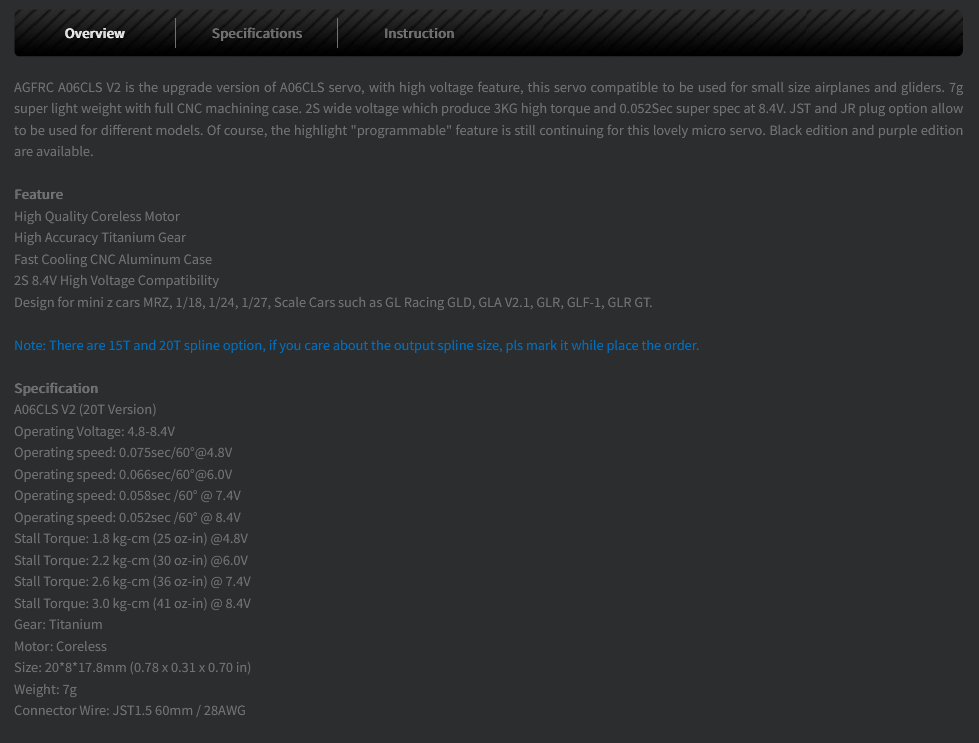
\includegraphics[width=\textwidth]{Images/A06_motor_info_curt.png}
    \caption{A06CLS V2 Motor Information (Curt)}
    \label{fig:A06CLS_V2_motor_info_curt}
\end{figure}

\begin{comment}
\subsection{A06CLS V2 Information Brochure}
\label{appendix:A06CLS_V2_brochure}

\begin{figure}[H]
    \centering
    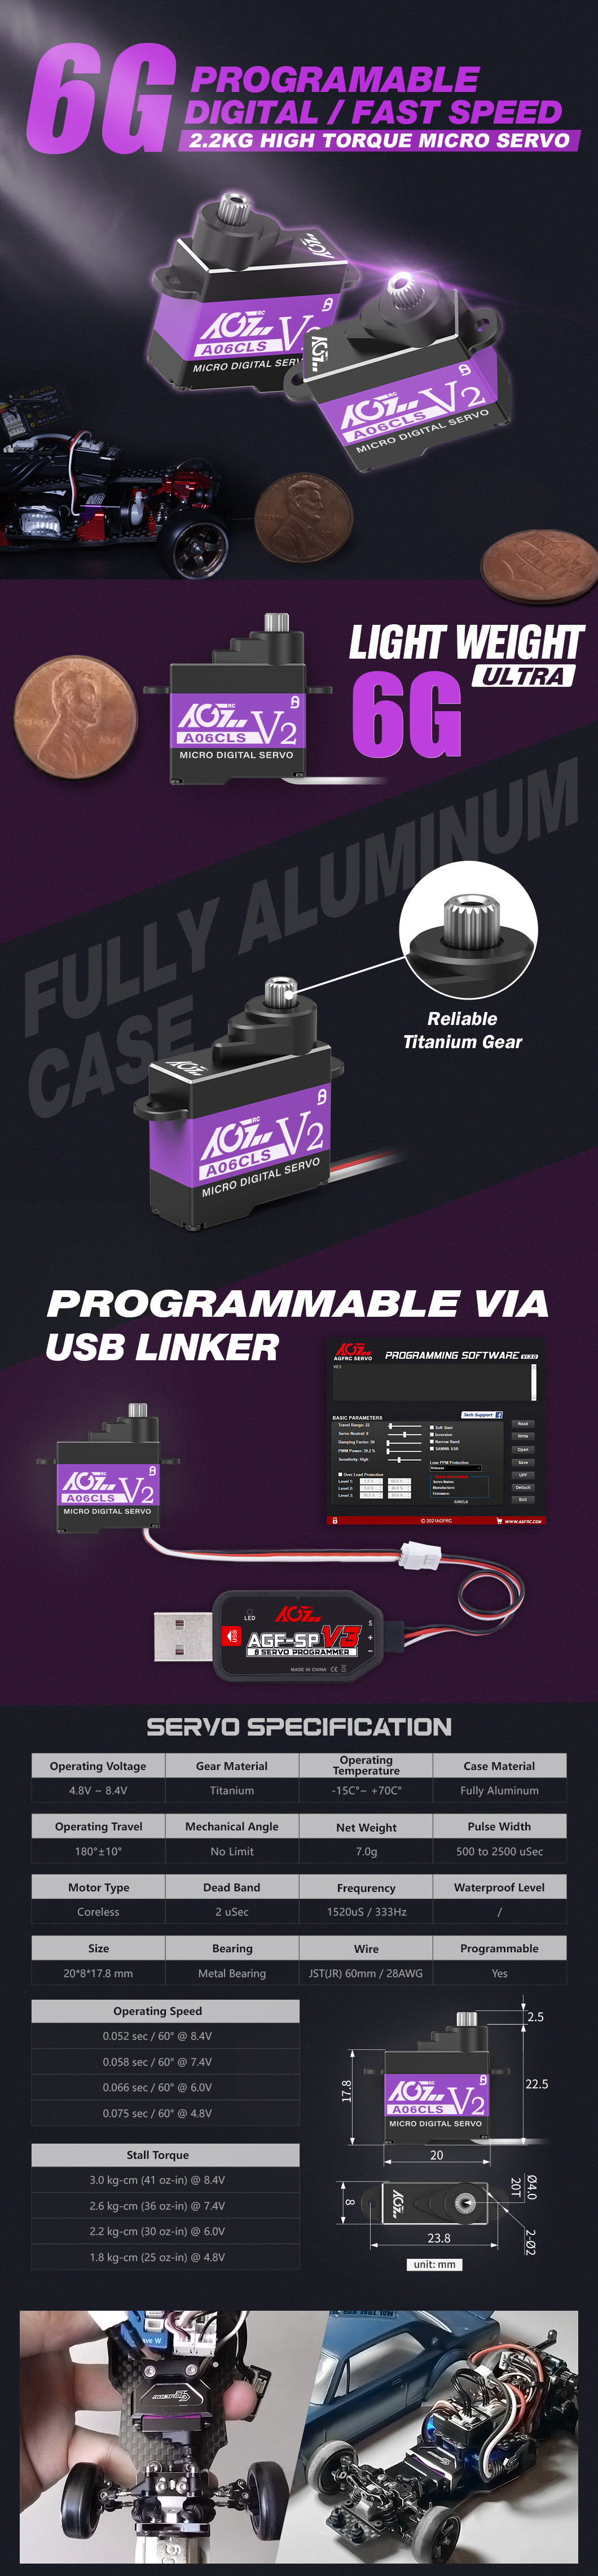
\includegraphics[width=0.5\textwidth]{Images/A06_motor_info.jpg}
    \caption{A06CLS V2 Motor Information}
    \label{fig:A06CLS_V2_motor_info}
\end{figure}
\end{comment}

\subsection{A20BHM Website Information}
\label{appendix:A20_info}

This information is taken from the website: \newline    
https://www.agf-rc.com/agfrc-a20bhm-21g-high-speed-0068sec-114kg-programmable-digital-brushless-48-84v-strength-steel-gear-micro-wing-servo-18010-for-airplane-aircraft-p4231199.html
\begin{figure}[H]
    \centering
    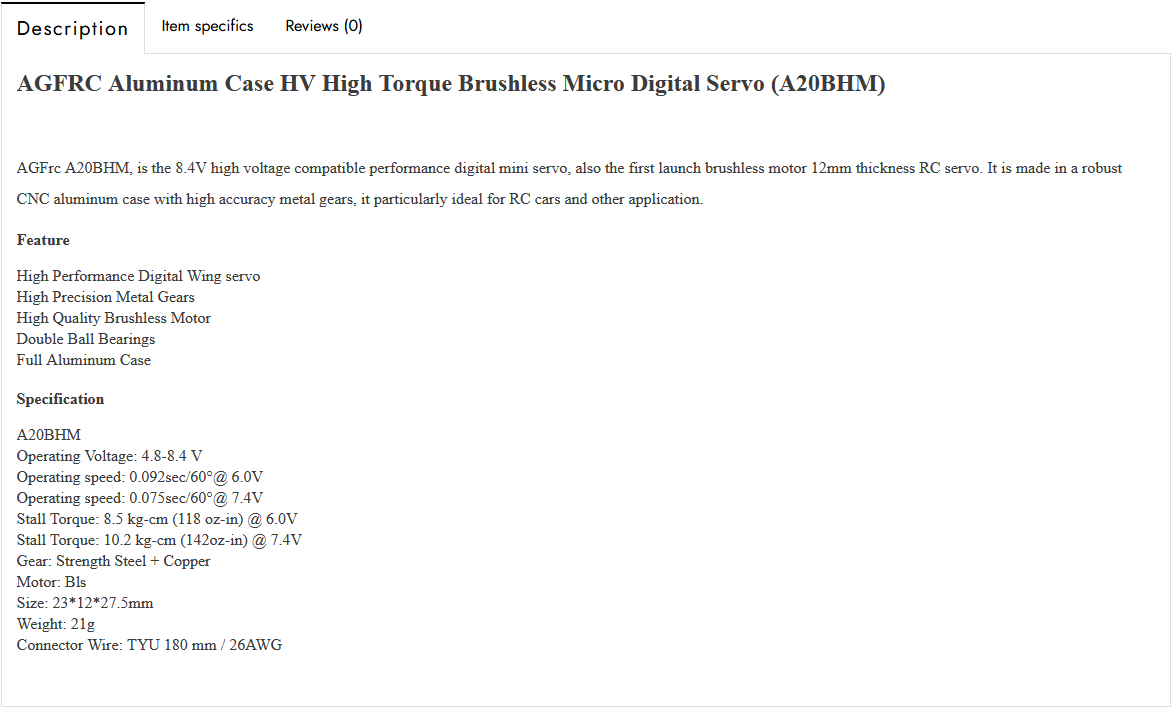
\includegraphics[width=\textwidth]{Images/A20_info.png}
    %\caption{A20 Information}
    \label{fig:A20_info}
\end{figure}

\subsection{A35CHM Motor Information}
\label{appendix:A35CHM_motor_info}

\begin{figure}[H]
    \centering
    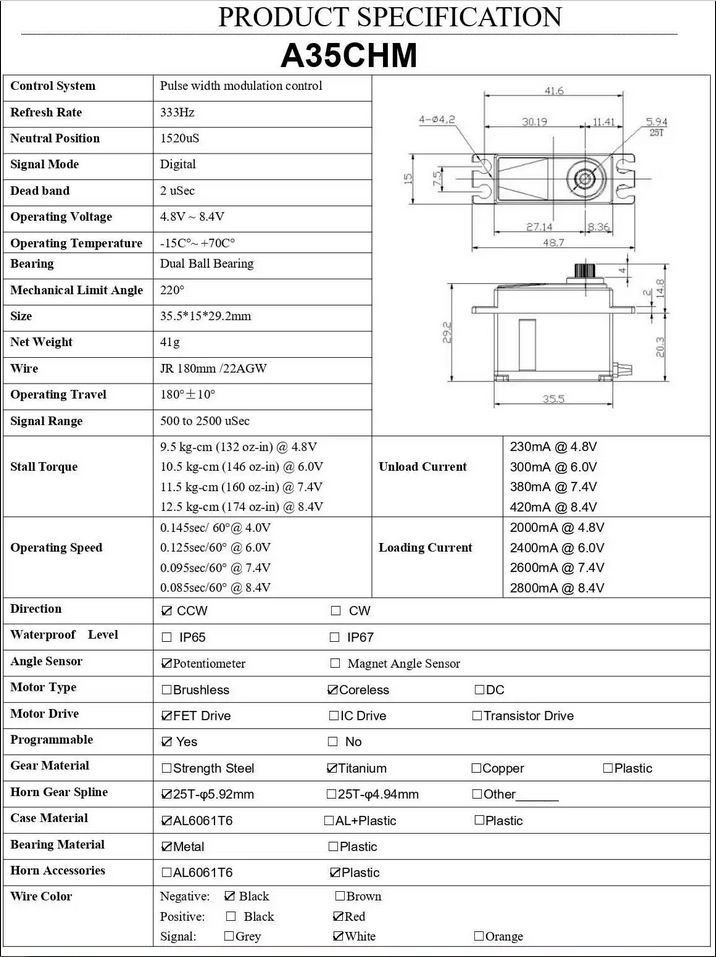
\includegraphics[width=\textwidth]{Images/A35CHM_info.png}
    \caption{A35CHM Motor Information}
    \label{fig:A35CHM_info}
\end{figure}

\subsection{A80BHP-H Motor Information}
\label{appendix:A80_motor_info}

Please note that this brochure gives an operating travel of 90 degrees, this was later confirmed to be false, the actual operating travel is 180 degrees.
\begin{figure}[H]
    \centering
    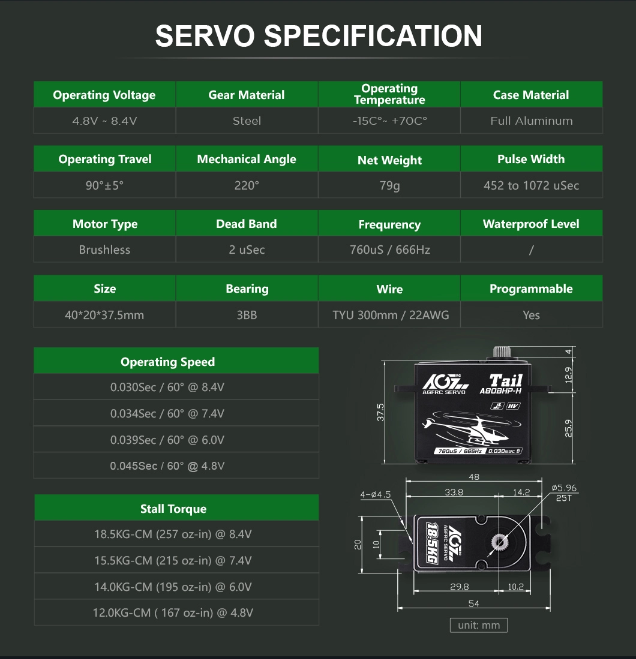
\includegraphics[width=\textwidth]{Images/A80_motor_info.png}
    \caption{A80BHP-H Motor Information}
    \label{fig:A80_motor_info}
\end{figure}

\subsection{Ultimaker Tough PLA Technical Data Sheet}
\label{appendix:tough_PLA}

\begin{figure}[H]
    \centering
    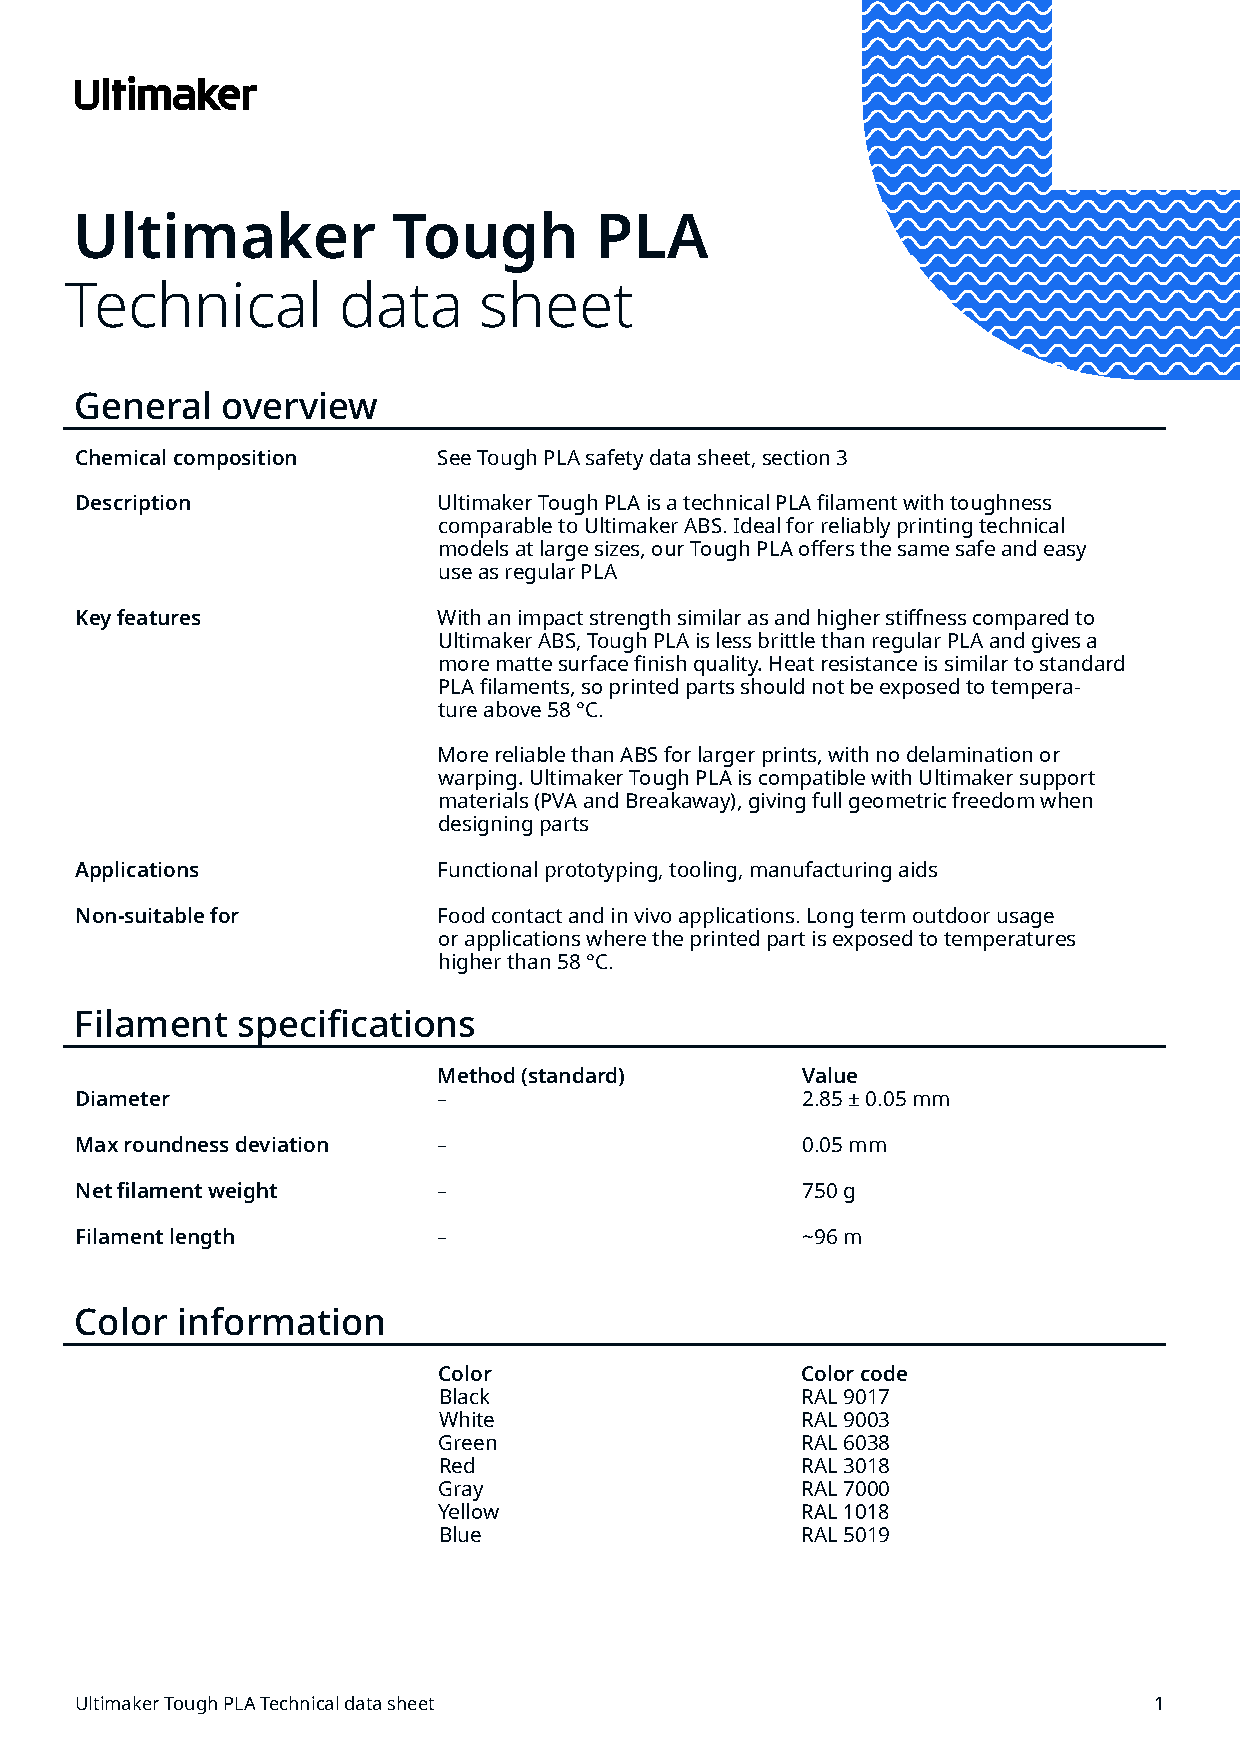
\includegraphics[width=\textwidth]{Images/UM220509-Tough-PLA-TDS-RB-v2.10.pdf}
    \caption{UM220509 Tough PLA TDS}
    \label{fig:tough_PLA}
\end{figure}